% $Id:
% !Mode:: "TeX:DE"    % Setting document mode and submode for WinEdt
% ..............................................................................
%             W A S  I S T  S A G E M A T H  ?
% ~~~~~~~~~~~~~~~~~~~~~~~~~~~~~~~~~~~~~~~~~~~~~~~~~~~~~~~~~~~~~~~~~~~~~~~~~~~~~~

\newpage
\hypertarget{appendix-using-sage}{}
\section{Kurzeinführung in das CAS SageMath}
\label{s:appendix-using-sage}
\index{SageMath}
\index{SageMath!Programmbeispiele}

%% Unter \url{https://wiki.sagemath.org/combinat} gibt es Weiterentwicklung on-top of Sage.
%% Diese kommen meist nach und nach ins offizielle Sage rein.


Dieses Buch enthält zahlreiche mit SageMath erstellte Programmbeispiele. SageMath ist
ein Open-Source Computer-Algebra-System (CAS), das für Lehre, Studium und Forschung
eingesetzt wird.
SageMath kombiniert viele hochwertige Open-Source-Packete\footnote{%
Einen Eindruck von der Größe von SageMath erhält man, wenn man es selbst compiliert:
Die heruntergeladenen Sourcen von SageMath 4.1 brauchten zur Compilierung auf einem
durchschnittlichen Linux-PC rund 5 h (inklusive aller Bibliotheken).
Danach nahm es 1,8 GB Plattenplatz ein.
}
und liefert den Zugang zu deren Funktionalität über ein gemeinsames, auf der
Programmiersprache Python\index{Python} basierendes Interface\footnote{%
Es gibt auch ein relativ einfaches Interface für die Sprache C, genannt Cython,
mit der man eigene Funktionen in SageMath stark beschleunigen kann.\\
Siehe \url{http://openwetware.org/wiki/Open_writing_projects/Sage_and_cython_a_brief_introduction}.
}.

\noindent SageMath kann man auf vielfältige Weise nutzen:
als mächtigen Taschenrechner; als Tool für das Mathematikstudium;
oder als Programmier-Umgebung, um Algorithmen zu prototypen oder um Forschung im
Bereich der algorithmischen Aspekte der Mathematik zu betreiben.

\noindent Einen schnellen Einstieg bieten z.B. die Referenzen in dieser Fußnote%
\footnote{%
\noindent\hangindent=6pt\makebox[6pt][l]{-}\glqq Einladung zu Sage\grqq~von David Joyner, letztes Update 2009,\\
  \url{http://sage.math.washington.edu/home/wdj/teaching/calc1-sage/an-invitation-to-sage.pdf}

\noindent\hangindent=6pt\makebox[6pt][l]{-}\glqq The SDSU Sage Tutorial\grqq,\\
  \url{http://www-rohan.sdsu.edu/~mosulliv/sagetutorial/}\\
  \url{http://www-rohan.sdsu.edu/~mosulliv/sagetutorial/sagecalc.html}

  \noindent\hangindent=6pt\makebox[6pt][l]{-}{\glqq SAGE For Newbies\grqq~von Ted Kosan, 2007,\\
  \url{http://sage.math.washington.edu/home/tkosan/newbies_book/sage_for_newbies_v1.23.pdf}}
   % Leerzeile am Ende nötig, sonst hat die letzte Zeile KEINEN hängenden Einzug?! (TODO_LaTeX)
   %%%% Aber das auch unschön.
}.

\noindent Die offizielle SageMath Online-Dokumentation\footnote{%
  Die entsprechenden offiziellen PDF-Dokuments können herunter geladen werden von\\
  \url{http://www.sagemath.org/help.html}, \url{http://www.sagemath.org/doc} und \url{http://planet.sagemath.org}.
} finden Sie unter: \url{http://www.sagemath.org}.


\noindent Es gibt inzwischen viele PDF- und HTML-Dokumente über SageMath, so dass wir als guten Startpunkt nur einige wenige nennen\footnote{%
- \glqq Bibliothek\grqq: {\centering \url{http://www.sagemath.org/library.html}},\\
- \glqq Dokumentationsprojekt\grqq:
  {\centering \url{http://wiki.sagemath.org/DocumentationProject}},\\
- \glqq Lehrmaterial\grqq: {\centering \url{http://wiki.sagemath.org/Teaching_with_SAGE}}.
}.

\noindent Auch beim Studium der Kryptologie können fertige SageMath-Module genutzt
werden\footnote{%
\noindent\hangindent=6pt\makebox[6pt][l]{-}Überblick,
   welche Kryptographie momentan in SageMath enthalten ist:\\
   \url{http://www.sagemath.org/doc/reference/sage/crypto/}

\noindent\hangindent=6pt\makebox[6pt][l]{-}Diskussionen
   über Lernaspekte beim Entwickeln weiterer Krypto-Module in SageMath:\\
   \url{http://groups.google.com/group/sage-devel/browse_thread/thread/c5572c4d8d42d081}
% Leerzeile bei den Aufzählungen am Ende nötig, damit die 2. Zeile (Url) hängenden Einzug hat.
% ABER: Bei der letzten Aufzählung führt Leerzeile zu leerer Zeile (was nicht gewollt ist) und die letzte Url hat trotzdem keinen hängenden Einzug! (TODOTODO)
}.

\noindent Umfangreiche Kryptographie-Einführungen finden sich in der folgenden Fußnote\footnote{%
\noindent\hangindent=6pt\makebox[6pt][l]{-}Ein fertiger Kryptographie-Kurs von David Kohel,
  der SageMath nutzt, aus 2008:\\
  {\centering \url{http://www.sagemath.org/files/kohel-book-2008.pdf} }\\
  bzw. derselbe Kurs in einer neueren Fassung (2015)\\
  {\centering \url{http://iml.univ-mrs.fr/~kohel/tch/M2-CryptoSymetrique/crypto.pdf} }.

\noindent\hangindent=6pt\makebox[6pt][l]{-}\glqq Introduction to Cryptography with
  Open-Source Software\grqq, ein hervorragendes Buch von Alasdair McAndrew, CRC, 2011
  %% TODO: Wenn die eine Zeile länger, beginnt sie doch wieder ganz vorne!
}.


% ---------------------------------------------------------------------------
\section*{SageMath-Benutzerschnittstellen}
SageMath ist kostenlos und kann von folgender Webseite herunter geladen werden:
\begin{center}
  \url{http://www.sagemath.org} \\
\end{center}
Standardmäßig nutzt man die SageMath-\textbf{Kommandozeile} als Interface, wie im
folgenden Bild~\ref{fig:sage_cmd_interfaces} zu sehen ist.
Es gibt jedoch auch ein grafisches Benutzerinterface für diese Software
in Form des SageMath-Notebooks (siehe Bild~\ref{fig:sage_gui_interfaces}).
Und schließlich kann man SageMath-\textbf{Notebooks}\footnote{%
Weitere Details zu SageMath-Notebooks finden Sie in
Kapitel~\ref{ec:Sage_Massierer}
(\glqq \nameref{ec:Implementing-for-Education}\grqq
  $\Rightarrow$ \glqq \nameref{ec:Sage_Massierer}\grqq).
                      }
auch online auf verschiedenen Servern nutzen, ohne SageMath lokal zu installieren, z.B.:
\begin{center}
\url{http://sagecell.sagemath.org/} oder \\
\url{https://cocalc.com/}
\end{center}

SageMath läuft unter den Betriebssystemen Linux, Mac OS X und Windows.
Auf der Windows-Plattform läuft die komplette SageMath-Distribution momentan
nur als ein VMware-Image.

\begin{figure}[!htpb]
\centering
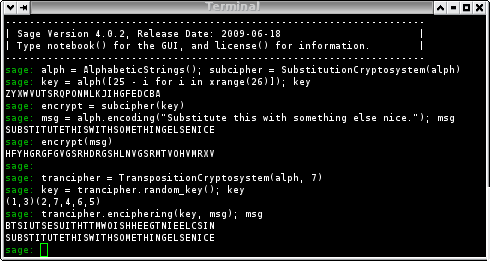
\includegraphics[scale=0.6]{figures/sage-cmd}
\caption{SageMath-Kommandozeilen-Interface}
\label{fig:sage_cmd_interfaces}
\end{figure}

\begin{figure}[!htpb]
\centering
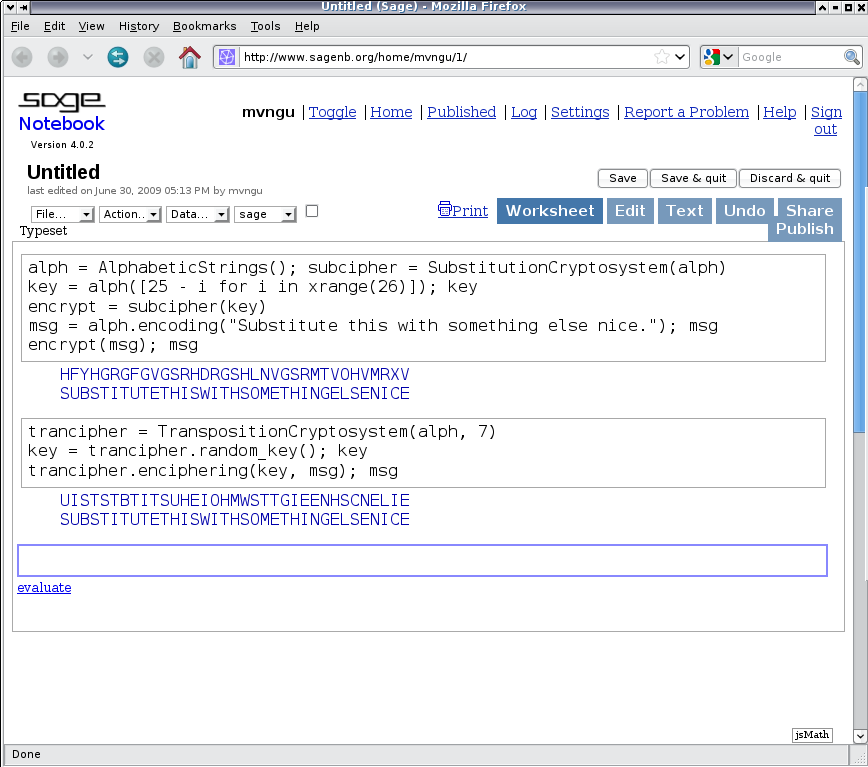
\includegraphics[scale=0.4]{figures/sage-gui}
\caption[SageMath-Notebook-Interface]{SageMath-Notebook-Interface\footnotemark}
\label{fig:sage_gui_interfaces}
\end{figure}

\footnotetext{%
Um das grafische SageMath-Interface lokal zu starten, muss man auf der SageMath-Kommandozeile
\verb#notebook()# eingeben. Danach startet der eingestellte Browser (Iceweasel,
Firefox, IE, ...) z.B. mit der URL \textit{http://localhost:8000}.
}



% ---------------------------------------------------------------------------
\newpage
\section*{Hilfe beim Benutzen von SageMath}

Wenn man SageMath auf der Kommandozeile startet, erhält etwas wie die folgenden Zeilen:
%
\begin{Verbatim}%
[fontsize=\footnotesize]
mnemonic:~$ sage
----------------------------------------------------------------------
| Sage Version 4.1, Release Date: 2009-07-09                         |
| Type notebook() for the GUI, and license() for information.        |
----------------------------------------------------------------------

sage: help
Type help() for interactive help, or help(object) for help about object.
sage:
sage:
sage: help()

Welcome to Python 2.6!  This is the online help utility.

If this is your first time using Python, you should definitely check out
the tutorial on the Internet at http://docs.python.org/tutorial/.

Enter the name of any module, keyword, or topic to get help on writing
Python programs and using Python modules.  To quit this help utility and
return to the interpreter, just type "quit".

To get a list of available modules, keywords, or topics, type "modules",
"keywords", or "topics".  Each module also comes with a one-line summary
of what it does; to list the modules whose summaries contain a given word
such as "spam", type "modules spam".
\end{Verbatim}
%
Viele weitere Hilfen gibt es als offizielle SageMath-Dokumentation, die mit jedem
Release von SageMath verteilt wird~(siehe Bild~\ref{fig:sage_standard_doc}).
%
\begin{figure}[!htpb]
\centering
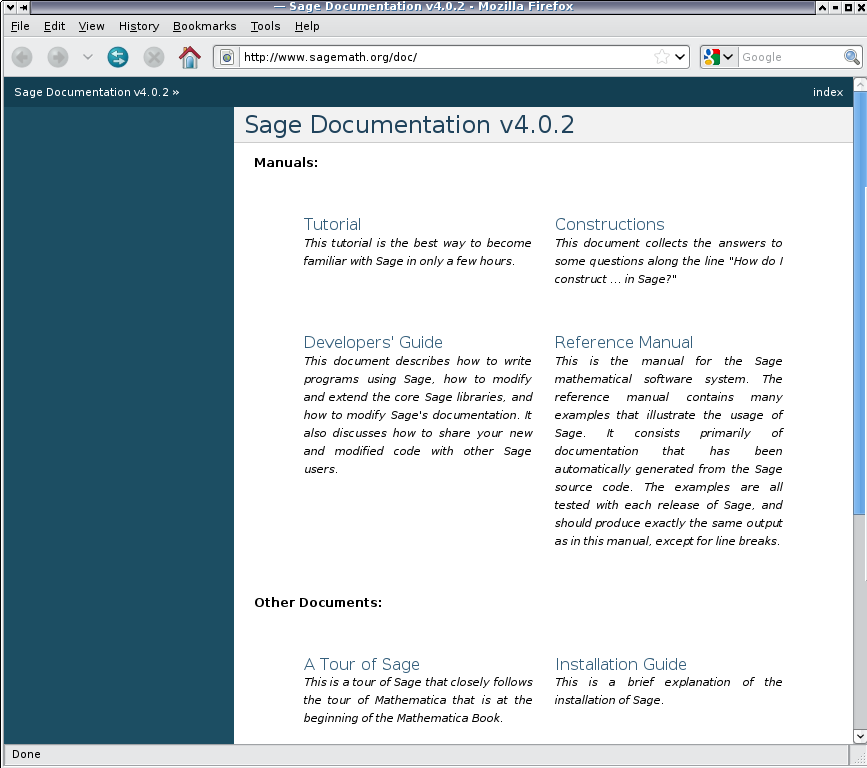
\includegraphics[scale=0.4]{figures/sage-online-doc}
\caption{Die Standard-Dokumentation von SageMath}
\label{fig:sage_standard_doc}
\end{figure}
%
Zur offiziellen SageMath-Standard-Dokumentation gehören folgende Dokumente:

\begin{itemize}
\item Tutorial --- Das Tutorial ist für SageMath-Einsteiger.
  Es ist dafür gedacht, sich in ein bis drei Stunden mit den
  wichtigsten Funktionen vertraut zu machen.

\item Constructions --- Dieses Dokument ist im Stil eines \glqq Kochbuchs\grqq~mit
  einer Sammlung von Antworten auf Fragen zur Konstruktion von SageMath-Objekten.

\item Developers' Guide --- Dieser Führer ist für Entwickler, die selbst SageMath
  mit weiter entwickeln wollen. Enthalten sind darin z.B. Hinweise zum
  Stil und zu Konventionen beim Programmieren, zur Modifikation von
  SageMath-Kern-Bibliotheken oder von SageMath-Standard-Dokumentation, und zum Code-Review
  und zur Software-Verteilung.

\item Reference Manual --- Dieses Handbuch enthält die komplette Dokumentation
  aller wichtigen SageMath-Funktionen. Zu jeder Klassen-Beschreibung gibt es
  mehrere Code-Beispiele. Alle Code-Beispiele im Referenz-Handbuch werden
  bei jedem neuen SageMath-Release getestet.

\item Installation Guide --- Dieser Führer erklärt, wie man SageMath auf
  verschiedenen Plattformen installiert.

\item A Tour of Sage --- Diese Tour durch SageMath zeigt exemplarisch verschiedene
  Funktionen, die für Einsteiger sinnvoll sind.

\item Numerical Sage --- Dieses Dokument führt Werkzeuge auf, die in SageMath
  für numerische Mathematik verfügbar sind.

\item Three Lectures about Explicit Methods in Number Theory Using
  Sage --- Drei Vorlesungen über Methoden der Zahlentheorie, die explizit
  SageMath nutzen. Dieses Dokument zeigt wie man mit SageMath Berechnungen in
  fortgeschrittener Zahlentheorie durchführt.
\end{itemize}

\noindent Von der SageMath-Kommandozeile erhält man eine Liste aller verfügbaren Kommandos
(Funktionsnamen etc.), die ein bestimmtes Muster haben, wenn man die ersten Zeichen tippt,
und dann die \glqq Tab\grqq-Taste drückt:
%
\begin{Verbatim}%
[fontsize=\footnotesize]
sage: Su[TAB]
Subsets                   Subwords                  SuzukiGroup
SubstitutionCryptosystem  SupersingularModule
\end{Verbatim}
%
Wenn man den genauen Namen eines Kommandos kennt, kann man die \texttt{help}-Funktion
nutzen oder das Fragezeichen \glqq ?\grqq~anfügen, um weitere Informationen zu
diesem Kommando zu erhalten.  Zum Beispiel liefert das Kommando
\texttt{help(SubstitutionCryptosystem)} die Dokumentation zur der eingebauten
Klasse \texttt{SubstitutionCryptosystem}. Mit dem Fragezeichen erhalten wir die
Dokumentation zu dieser Klasse auf folgende Weise:
%
\begin{Verbatim}%
[fontsize=\footnotesize]
sage: SubstitutionCryptosystem?
Type:type
Base Class:<type 'type'>
String Form:<class 'sage.crypto.classical.SubstitutionCryptosystem'>
Namespace:Interactive
File:/home/mvngu/usr/bin/sage-3.4.1/local/lib/python2.5/site-packages/sage/crypto/classical.py
Docstring:

        Create a substitution cryptosystem.

        INPUT:

        - ``S`` - a string monoid over some alphabet

        OUTPUT:

        - A substitution cryptosystem over the alphabet ``S``.

        EXAMPLES::

            sage: M = AlphabeticStrings()
            sage: E = SubstitutionCryptosystem(M)
            sage: E
            Substitution cryptosystem on Free alphabetic string monoid
            on A-Z
            sage: K = M([ 25-i for i in range(26) ])
            sage: K
            ZYXWVUTSRQPONMLKJIHGFEDCBA
            sage: e = E(K)
            sage: m = M(``THECATINTHEHAT'')
            sage: e(m)
            GSVXZGRMGSVSZG

        TESTS::

            sage: M = AlphabeticStrings()
            sage: E = SubstitutionCryptosystem(M)
            sage: E == loads(dumps(E))
            True
\end{Verbatim}
%
\vspace{30pt}
Weitere Unterstützung für spezifische Probleme gibt es in den Archiven der
\texttt{sage-support} Mailing-Liste unter
%
\begin{center}
  \url{http://groups.google.com/group/sage-support}
\end{center}




% ---------------------------------------------------------------------------
\newpage
\section*{Beispiele für in SageMath eingebaute mathematische Funktionen}

Hier sind ein paar kleine Beispiele\footnote{%
Diese Beispiele stammen aus einem nicht mehr existierenden Blog aus 2008 von Dr. Alasdair McAndrew.
%%%, Victoria University
%%%,\\ \url{http://amca01.wordpress.com/2008/12/19/sage-an-open-source-mathematics-software-system}
}
(alle für das Kommandozeilen-Interface -- zur einfacheren Nutzung), um zu sehen,
was man mit SageMath machen kann:

\begin{sagecode}
\begin{Verbatim}%
[fontsize=\footnotesize]
# * Analysis (Infinitesimalrechnung):
    sage: x=var('x')
    sage: p=diff(exp(x^2),x,10)*exp(-x^2)
    sage: p.simplify_exp()
     1024 x^10 + 23040 x^8 + 161280 x^6 + 403200 x^4 + 302400 x^2 + 30240

# * Lineare Algebra:
    sage: M=matrix([[1,2,3],[4,5,6],[7,8,10]])
    sage: c=random_matrix(ZZ,3,1);c
     [ 7 ]
     [-2 ]
     [-2 ]
    sage: b=M*c
    sage: M^-1*b
     [ 7 ]
     [-2 ]
     [-2 ]

# * Zahlentheorie:
    sage: p=next_prime(randint(2^49,2^50));p
      1022095718672689
    sage: r=primitive_root(p);r
      7
    sage: pl=log(mod(10^15,p),r);pl
      1004868498084144
    sage: mod(r,p)^pl
      1000000000000000

# * Endliche Körper (\url{http://de.wikipedia.org/wiki/Endlicher_K%C3%B6rper}):
    sage: F.<x>=GF(2)[]
    sage: G.<a>=GF(2^4,name='a',modulus=x^4+x+1)
    sage: a^2/(a^2+1)
      a^3 + a
    sage: a^100
      a^2 + a + 1
    sage: log(a^2,a^3+1)
      13
    sage: (a^3+1)^13
      a^2
\end{Verbatim}
\caption{Einige kleine Beispiele in SageMath aus verschiedenen Gebieten der Mathematik}
\end{sagecode}



% ---------------------------------------------------------------------------
\newpage
\section*{Programmieren mit SageMath}

Wenn man ein CAS (Computer-Algebra-System) nutzt, schreibt man zu Beginn einzelne
Befehle in die Kommandozeile wie im obigen Beispiel\footnote{%
  Standardmäßig wird SageMath-Code auch so präsentiert: Dabei beginnen die Zeilen
  mit  \glqq sage:\grqq~und \glqq ...\grqq.
  \begin{Verbatim}%
  [fontsize=\footnotesize]
  sage: m = 11
  sage: for a in xrange(1, m):
  ....:     print [power_mod(a, i, m) for i in xrange(1, m)]
  ....:
  \end{Verbatim}

  \noindent Auch dieses Skript benutzt normalerweise die obige Konvention, um
  SageMath-Code zu präsentieren, solange der Code nicht aus einer SageMath-Skriptdatei kommt.
  Wenn man den SageMath-Code aus diesem Skript kopiert und per Paste auf der SageMath-Kommandozeile
  wieder einfügt, sollte man \glqq sage:\grqq~und \glqq ...\grqq~ weglassen
  (obwohl das Kommandozeilen-Interface in den meisten Fällen mit diesen Präfixen
  korrekt umgehen kann).}.

Wenn man eigene Funktionen entwickelt, sie ändert und aufruft, dann ist es viel einfacher,
die Entwicklung in einem eigenen Editor vorzunehmen, den Code als SageMath-Skriptdatei zu
speichern und die Funktionen nicht-interaktiv auf der Kommandozeile auszuführen.
Beide Arten, Code zu entwickeln, wurden in
Kapitel \ref{CM_Sage_samples} (\glqq \nameref{CM_Sage_samples}\grqq),
Kapitel \ref{PaP_Sage_samples} (\glqq \nameref{PaP_Sage_samples}\grqq),
Kapitel \ref{primes:_Appendix_Sage-Samples} (\glqq \nameref{primes:_Appendix_Sage-Samples}\grqq)
und in Kapitel \ref{NumberTheory_Appendix_E} (\glqq\nameref{NumberTheory_Appendix_E}\grqq)
angewandt.

\noindent Um SageMath-Code in einem eigenen Editor zu entwickeln und zu testen, gibt es zwei
nützliche Befehle: \verb!load()! und \verb!attach()!\footnote{%
Vergleiche das SageMath-Tutorial über Programmierung, Kapitel
\glqq Loading and Attaching Sage files\grqq,\\
\url{http://doc.sagemath.org/html/en/tutorial/programming.html}.}.\\
Angenommen Sie haben die folgende Funktions-Definition:
\begin{Verbatim}%
   [fontsize=\footnotesize]
   def function(var1):
       r"""
       DocText.
       """
       ...
       return (L)
\end{Verbatim}
\noindent die in der Datei \texttt{primroots.sage} gespeichert wurde.

\noindent Um diese Funktion in SageMath zu laden (und syntaktisch gleich zu testen),
wird der Befehl \verb!load()! benutzt:

\texttt{sage: load primroots.sage}

\noindent Danach kann man auf der Kommandozeile alle Variablen und Funktionen
nutzen, die im Sage\-Math-Skript definiert wurden\footnote{%
Anmerkungen:

\noindent\hangindent=6pt\makebox[6pt][l]{-}Bitte keine Leerzeichen
oder White Spaces im Dateinamen.

\noindent\hangindent=6pt\makebox[6pt][l]{-}Es empfiehlt sich,
der SageMath-Skriptdatei die Datei-Extension
\glqq .sage\grqq~statt \glqq .py\grqq~zu geben.
Hat ein SageMath-Skript die Dateinamens-Endung \glqq .sage\grqq, dann wird
beim Laden der Datei in SageMath auch gleich die normale SageMath-Umgebung mit geladen,
um die Syntax zu prüfen. Genauso funktioniert es, wenn man ein SageMath-Skript direkt
von einer Bash-Shell aufruft mit~~\texttt{\$ sage primroots.sage}.

\noindent\hangindent=6pt\makebox[6pt][l]{-}Beim Laden des obigen
SageMath-Skripts wird es von SageMath zuerst geparst, und dann
in eine andere Datei namens \glqq primroots.py\grqq~kopiert. SageMath ergänzt
dann alle notwendigen Variablen in \glqq primroots.py\grqq~und alle Import-Statements.
Somit wird das SageMath-Skript genauso ausgeführt, als hätte man die Befehle einzeln
auf der Kommandozeile eingetippt. Ein bedeutender Unterschied ist,
dass alle Ausgaben ein \verb!print!~benötigen.

}.

Normalerweise editiert man ein eigenes SageMath-Skript wieder und möchte dann den
Inhalt des geänderten Skripts wieder in SageMath laden. Dafür kann man den Befehl
\verb!attach()! nutzen (man kann auch direkt nach dem \verb!load()!
das \verb!attach()! aufrufen, und nicht erst, wenn man das Skript ändert;
man kann \verb!load()! sogar weglassen, da dies in \verb!attach()! enthalten ist):

\texttt{sage: attach primroots.sage}

Nun kann man das SageMath-Skript ändern und die geänderte Funktionsdefinition
wird -- solange man die SageMath-Session nicht beendet -- beim nächsten Enter
in SageMath geladen (und syntaktisch gleich geprüft). Diese Neuladen passiert
vollkommen automatisch. Der Befehl attach() lässt SageMath also permanent die
genannte Datei auf Änderungen überwachen. Damit spart man sich das Kopieren
und Pasten zwischen dem eigenen Texteditor und dem SageMath-Kommandozeilen-Interface.

Hier ist ein Bild, das SageMath-Code im Editor GVIM zeigt -- mit aktiviertem
Syntax-Highlighting (siehe Bild~\ref{fig:sage-highlighted-code-in-editor}).
%
\begin{figure}[!htpb]
\centering
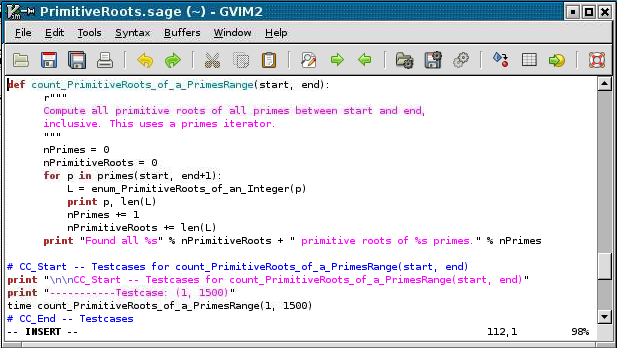
\includegraphics[scale=0.7]{figures/sage-highlighted-code-in-editor}
\caption{SageMath-Beispiel in einem Editor mit aktiviertem Code-Highlighting}
\label{fig:sage-highlighted-code-in-editor}
\end{figure}

\vspace{20pt}
Falls man die Ausgabe einer attachten Datei so angezeigt haben möchte,
wie wenn man die Einzelbefehle direkt auf der Kommandozeile eingibt
(also nicht nur das, was per \verb!print! ausgegeben wird),
kann man den Befehl \verb!iload()! verwenden:
Jede Zeile wird dann einzeln geladen. Um die nächste Zeile zu laden,
muss man die \verb!Enter!-Taste drücken. Das muss man so lange wiederholen,
bis alle Zeilen des SageMath-Skripts in die SageMath-Session geladen sind.

\texttt{sage: iload primroots.sage}


% \vspace{30pt}
\newpage
\noindent Weitere Hinweise:
\begin{itemize}
  \item Abfrage der Version Ihrer SageMath-Umgebung mit: \texttt{version()}
  \item Um sich schnell die SageMath-Programmbeispiele in diesem Skript anzusehen, können Sie
    \begin{itemize}
      \item im Index nach \verb#SageMath -> Programmbeispiele# schauen, oder
      \item sich im Anhang das \glqq \nameref{sc:List-of-Sage-Code-Examples}\grqq~ansehen.
    \end{itemize}
  \item Die SageMath-Beispiele in diesem Skript werden mit CrypTool ausgeliefert.\\
        Weitere Details am Ende der Übersicht
        \glqq \nameref{sc:List-of-Sage-Code-Examples}\grqq.
\end{itemize}


